\documentclass[a4paper, 11pt]{article}
\usepackage[slovene]{babel}
\usepackage[utf8]{inputenc}
\usepackage{graphicx}
\usepackage{fancyhdr}
\usepackage{biblatex}
\usepackage{enumerate}
\usepackage[normalem]{ulem}
\usepackage{amsmath,amsthm,amssymb}
\usepackage{algorithmic}
\newtheorem{example}{Primer}
\usepackage{graphicx}
\usepackage{tabularx}
\usepackage{amsfonts}
\usepackage{eurosym}
\usepackage{tikz}
\usetikzlibrary{fadings,positioning,calc}
\tikzset{
	casual/.style={
	rectangle,
	draw=black, very thick,
	text width=6.5em,
	minimum height=2em,
	text centered
	}}
\newtheorem{theorem}{Trditev}
\newtheorem{definition}{Definicija}
\newtheorem{corollary}{Primer}


	\begin{document}
		\begin{titlepage}
			\begin{center}

			\large
			Univerza v Ljubljani\\
				\normalsize
				Fakulteta za matematiko in fiziko\\

			\vspace{5 cm} 

				\large
				Finančni praktikum\\


			\vspace{0.5cm}
			\LARGE
				\textbf{Algoritem za reševenje dvostopenjskega problema nahrbtnika z dinamičnim programiranjem}

			\vspace{0.5 cm}

			\large
				Jakob Zarnik, Tin Markon \\


			\vspace{1.5cm}
			\normalsize
				Mentorja: prof. dr. Sergia Cabello Justo, asist. dr. Janoš Vidali
			\vspace{3cm}


			\vfill

				\large Ljubljana, 2020

			\end{center}
		\end{titlepage}


\newpage

\tableofcontents
\vspace{22mm}

\newpage
		
	\pagestyle{fancy}
	\fancyhead{}
	\fancyhead[R]{Dvostopenjski problem nahrbtnika}
	\fancyfoot{}
	\fancyfoot[R]{\thepage}
	\fancyfoot[L]{Jakob Zarnik, Tin Markon}
	
	\begin{abstract}
	
	V nalogi obravnavava reševanje dvostopenjskega problema nahrbtnika z dinamičnim programiranjem. Najprej problem opiševa in ga teoretično formulirava, nato pa za reševanje izdelava algoritem v programskem jeziku \textit{Python}. Preizkusiva ga na primerih z znano rešitvijo in izmeriva njegovo časovno zatevnost na naključno generiranih podatkih.
	
	\end{abstract}
	
	\pagebreak
	
	\section{Uvod}
	
	Dvostopenjski programi omogočajo modeliranje situacij, kjer glavni odločevalec, v nadaljevanju poimenovan investitor, optimizira svoja sredstva s tem, da neposredno upošteva odziv posrednika na njegovo odločitev o višini vložka. V primeru dvostopenjskega problema nahrbtnika (Bilevel Knapsack Problem), v nadaljevanju BKP, investitor določi prostornino nahrbtnika z namenom maksimizacije dobička, med tem ko se posrednik sooča z 0-1 problemom nahrbtnika s prostornino določeno s strani investitorja. BKP je ustrezen za modeliranje problema »ustreznega financiranja«, kjer posameznik (tj. investitor), svoja sredstva razdeli med netvegano naložbo s fiksnim donosom (npr. varčevalni račun, državna obveznica) in bolj tvegano naložbo, preko posrednika kot je banka ali bančni posrednik (broker). Ta kupi delnice ali obveznice z namenom maksimizacije svojega dobička s tem, da upošteva omejitve finančnih sredstev (prostornina nahrbtnika) investitorja in ustvari donos z ustrezno izbiro investicij. Podobno uporabo modeliranja lahko opazimo na področju upravljanja s proizvodi, kjer se podjetje odloča koliko enot izdelkov naj proda samo in koliko preko posrednika.
	
	BKP je mešan celoštevilski dvostopenjski problem predstavljen s strani Dempe in Richter, ki sta za rešitev predstavila "branch-and-bound" okvir (tj. razveji in omeji). V najini nalogi najprej razširiva potrebne in zadostne pogoje za obstoj optimalne rešitve. Nato predlagava enostaven in učinkovit algoritem dinamičnega programiranja za reševanje problema. V nasprotju s pristopom Dempe in Richter, kjer je beležen seznam nedominantnih rešitev, tukaj beležimo samo ciljne funkcijske vrednosti za oba, investitorja in posrednika, tekom dinamičnega procesa.
		
	\section{Formulacija in lastnosti problema}
	
	V narbtnik s prostornino oz kapaciteto $y$, ki jo določi investitor, vsakemu predmetu $j$ določimo utež oz. volumen $a_j$, zaslužek posrednika $c_j$ in zaslužek investitorja $d_j$. Ceno enote prostornine nahrbtnika označimo s $t$. Z danim $y$, posrednik izbere podmnožico predmetov, ki upošteva prostosrsko omejitev. To nam da dvostopenjski program
	\[   
	\text{BKP} = 
    	\begin{cases}
	 	\text{$\underset{y,x}{\text{Max}} f^{1}(y,x)=dx+ty$} \\
       		\text{s.t. $\underline{b} \leq y \leq \overline{b}$} \\
       		\text{$\underset{x}{\text{Max}} f^{2}(x)=cx$} \\
       		\text{s.t. $ax \leq y$ and $x \in \{ 0, 1\}^n$} \\ 
    	\end{cases}
	\]

	
kjer so $a$, $c$ in $d$ celoštevilske vrednosti in $a$, $c$, $d$, $\underline{b}$ in $\overline{b}$ nenegativne. V najini nalogi so z
	
	$$ \text{S} = \{ (x, y) \in \{ 0, 1 \}^n \times \left[ \underline{b}, \overline{b} \right]: ax \leq y\} $$ 
	
	označene omejitve, s 
	
	$$ \text{P}(y) = \{ x \in \text{Arg}\max \{ cx^\prime: ax^\prime \leq y, x^\prime \in \{ 0,1\}^n \} \}$$
	
	označimo posrednikovo racionalno izbiro množice (za fiksen $y$) in z 
	
	$$ \text{IR} = \{ (x,y)  | (x,y) \in S, x \in \text{P}(y) \} $$
	
	induktiven del, preko katerega investitor optimizira svojo funkcijo.
	
	Dvostopenjski program obstaja v dveh različicah. Optimističen primer, ko racionalna množica ni singelton (enolična), posrednik izbere tisto rešitev, ki maksimizira zaslužek investitorja. Dobljena rešitev se imenuje močna rešitev. V pesimističnem primeru pa investitor predvideva, da kadar ima posrednik več enakovrednih možnosti izbire množice, izbere tisto, ki minimizira investitorjev zaslužek. Tako dobimo šibko rešitev.
	
	\begin{theorem}[Dempe in Richter]
	Če je cena enote prostornine (enota $t$) nepozitivna, potem obstaja optimalna rešitev BKP.
	\label{trditev1}
	\end{theorem}
	
	Naslednja trditev povezuje ceno prostornine z investitorjevim razmerjem med zaslužkom in utežjo predmeta.
	
	\begin{theorem}
	Naj bo $\underline{b} = 0$ in $t < 0$. Če je  $| t | > \underset{1 \leq j \leq n}{max}(\frac{d_j}{a_j})$,  potem je $(y^*, x^*) = (0, 0_n)$ optimalna rešitev.
	\end{theorem}
	
	\begin{proof}
	Naj bo $(x, y)$ možna rešitev za dan BKP. Najprej z razširitvijo pogoja $ ax \leq y$ s $t$ $(t < 0)$ dobimo $(ta + d)x \geq ty + dx = f^{1}(y,x)$. Nato, ker je $ta_j + d_j < 0$ za $j = 1, \dots , n$ in $ x \in \{0, 1 \}^n$, sledi, da je $(ta + d)x \leq 0$, torej $f^{1}(y,x) \leq 0$. Vidimo, da ker je $(y^*, x^*) = (0, 0_n)$ možna rešitev danega BKP, v katerem je $f^{1}(y,x) = 0$, je ta rešitev tudi optimalna.
	\end{proof}
	
	Če je $\infty > \overline{b} \geq \sum_{i=1}^na_i$ in $t > 0$, potem je optimalna rešitev trivialna: $x^* = (1, \dots, 1)$ in $y^* = \overline{b}$. Če sta $d$ in $c$ kolinearna ($d = \alpha c$, kjer $\alpha > 0$) in $t \geq 0$, potem je reševanje BKP enako reševanju problema nahrbtnika s kapaciteto $\overline{b}$ za posrednika.
	
	\begin{definition}
	Diskreten dvostopenjski problem nahrbtnika (BKPd) je dvostopenjski problem nahrbtnika v katerem je spremenljivka, ki jo določi investitor diskretna.
	\end{definition}

	\begin{theorem}
	Če je $t \leq 0$, potem je vsaka optimalna rešitev $(y^*, x^*)$ za BKPd, tudi optimalna rešitev za BKP.
	
	Če je $t > 0$ in če optimalna rešitev za BKP obstaja, potem je optimalna tudi za BKPd.	
	\end{theorem}
	
	\begin{proof}
	$t \leq 0$: Iz \textbf{Trditve 1} sledi, da optimalna rešitev $(y^*, x^*)$ obstaja. Dodatno, IR (BKPd) $\subset$ IR (BKP) in iz Dempe in Richter sledi, da je $y^*$ celo število.
	
	$t > 0$: Direktno iz $(ii)$ v Dempe in Richter.
	\end{proof}

	Iz \textbf{Trditve 3} sledi, da je reševanje BKP ekvivalentno reševanju BKPd, ko je $t$ negativen. Če je $t$ pozitiven in optimalna rešitev obstaja (glej Izrek 4 v Dempe in Richter), je ta dosežena v točki $(\overline{b}, x^*)$, kjer je $x^* \in P(\overline{b})$. Pomni, da optimalna rešitev BKPd vedno obstaja. Torej, če BKP ima optimalno rešitev, to lako dobimo z reševanjem zaporedja problemov nahrbtnika, ki vsebuje binarne spremenljivke, eno za vsak možno vrednost $y$. Algoritem, opisan v naslednjem poglavju, uporabi to lastnost.
	
	\section{Opis programa}
	
	S programskim jezikom $Python$ sva napisala program, ki s pomočjo dinamičnega programiranja izračuna optimalno rešitev $(y^*, x^*)$ glede na naključno generirane podatke. S pomočjo primerov iz dokumenta sva preverila, če program deluje pravilno. Z uporabo algoritma lahko izračunamo rešitev tako v primeru optimističnega, kot tudi pesimističnega primera. V najslabšem scenariju ima časovno zahtevnost $\theta(n\overline{b})$, kar v zadnjem poglavju, s testom na naključnih podatkih, tudi pokaževa. Iz \textbf{Trditve 3} je razvidno, da je reševanje problema BKP ekvivalentno reševanju posrednikovega problema nahrbtnika za vsako celo število iz intervala $[ \underline{b}, \overline{b}]$. Algoritem v svojem teku jemlje obe ciljni funkciji. To dosežemo z dvema fazama, ki sta podrobneje opisani spodaj. \\

	\textbf{Forward phase} \\
	Prva faza je sestavljena iz dveh zank: zunanja zanka s koraki $k \in \left[1, \dots , n \right]$ in notranja zankna vezana na celoštevilsko kapaciteto nahrbtnika $y \in \left[ \underline{b}, \overline{b} \right]$. Med to fazo sta generirani dve tabeli. Prva vsebuje optimalne vrednosti sledilca
	$$ f^{2}_{k}(y) = max \left\{ \sum_{j=1}^{k} c_j x_j : \sum_{j=1}^{k} a_j x_j \leq y, x \in \{0, 1\}^k \right\} $$
	
	druga pa optimalne vrednosti investitorja
	$$ \widetilde{f}^{1}_{k}(y) = max \left\{ \sum_{j=1}^{k} d_j x_j : x \in P(y) \right\} $$
	
	na vsakem koraku $k$ in za vsako kapaciteto $y$. Za graditev teh tabel z dinamicnim programiranjem se rekurzija izvede za vse vrednosti $y$ med $0$ in $\overline{b}$ in za vsak predmet. Opomniti je treba, da funkcija  $\widetilde{f}^{1}_{k}(y)$ ne upošteva ceno prostornine nahrbtnika, in je torej   $\widetilde{f}^{1}_{k}(y) = f^{1}_{k}(y)+ty$. \\

	\begin{figure}[ht]
  	\centering
  		\begin{minipage}{0.9\linewidth}
			\begin{algorithmic}[1]
				\FOR{$k = 2, \dots, n$ \textbf{and} $y = 0, \dots \overline{b}$}
   					\IF{$y < a_k$}
						\STATE $f_{k}^{2}(y) = f_{k-1}^{2}(y)$ \textbf{and} $\widetilde{f}_{k}^{1}(y) = \widetilde{f}_{k-1}^{1}(y)$
					\ELSE
						\STATE $f_{k}^{2}(y) = max( f_{k-1}^{2}(y), f_{k-1}^{2}(y - a_k) + c_k)$
						\IF{$f_{k-1}^{2}(y) \neq f_{k-1}^{2}(y - a_k) + c_k$}
							\STATE $\widetilde{f}^{1}_{k}(y) = \widetilde{f}^{1}_{k-1}(y)$ \textbf{if} $f_{k}^{2}(y) = f_{k-1}^{2}(y)$
							\STATE $\widetilde{f}^{1}_{k}(y) = \widetilde{f}^{1}_{k-1}(y-a_k) + d_k$ \textbf{if} $f_{k}^{2}(y) = f_{k-1}^{2}(y - a_k) + c_k$
						\ELSE
							\STATE $\widetilde{f}^{1}_{k}(y) = max(\widetilde{f}^{1}_{k-1}(y), \widetilde{f}^{1}_{k-1}(y-a_k) + d_k)$ (Opt.)
							\STATE $\widetilde{f}^{1}_{k}(y) = min(\widetilde{f}^{1}_{k-1}(y), \widetilde{f}^{1}_{k-1}(y-a_k) + d_k)$ (Pes.)
						\ENDIF
					\ENDIF
				\ENDFOR
			\end{algorithmic}
		\end{minipage}
	\end{figure}
	
	V prvem koraku (tj. $k=1$) gledamo samo prvi predmet $x_1$. Optimalna rešitev investitorja in sledilca, za vsako kapaciteto y, je izračunana na sledeč način:
	\[   
	\text{$f_{1}^{2}(y) =$}
    	\begin{cases}
	 	\text{0 for $y = 0, \dots, a_1 - 1$} \\
       		\text{$c_1$ for $y = a_1, \dots, \overline{b}$} \\
    	\end{cases}
	\]
	
	\[   
	\text{$\widetilde{f}^{1}_{1}(y) =$}
    	\begin{cases}
	 	\text{0 for $y = 0, \dots, a_1 - 1$} \\
       		\text{$d_1$ for $y = a_1, \dots, \overline{b}$} \\
    	\end{cases}
	\]
	Sledilec izbere prvi predmet, samo če je dana kapaciteta zadostna. Funkcija za prvi korak je poimenovana \texttt{prvi\_predmeti} in se nahaja v datoteki \texttt{BKP.py}.
	
	Za $k > 1$ se za generiranje sledilčeve tabele uporabi rekurzija v 3. vrstici algoritma. Investitorjeva tabela je generirana glede na moč seznama sledilčeve optimalne rešitve. Če je sledilčeva rešitev enolična, je investitorjeva funkcija dana 7. in 8. vrstici, v nasprotnem primeru pa v 10. (optimističen scenarij) ali 11. (pesimističen scenarij) vrstici. 
	
	Funkcijo opisano z zgornjo psevdokodo sva poimenovala \texttt{generiranje\_tabel} se nahaja v datoteki \texttt{BKP.py}. Vrne nam dva seznama $n$ seznamov, prvega za investitorja in drugega za sledilca. \\
	
	\textbf{Backtracking phase} \\
	Druga faza je uporabljena za iskanje optimalne rešitve $(y^*, x^*)$, ki ustreza optimalni vrednosti določeni v prejšnji fazi. Optimalna kapaciteta $y$ je generirana z n-tim stolpcem tabele investitiorja (Opozoriti je potrebno, da se v programskem jeziku \textit{Python} indeksi elementov seznama začnejo z 0. Uporabila sva tabele velikosti $n \times (n+1)$, torej dejansko gledamo $(n+1)-ti$ stolpec.), kot je opisano v naslednji trditvi.
	
	\begin{theorem}
	Naj bo $(x^*, y^*)$ optimalna rešitev BKPd.
	\begin{itemize}
		\item Če je $t \leq 0$, potem $\widetilde{f}^{1}_{n}(y^*) + ty^* = Max \left\{ \widetilde{f}^{1}_{n}(y^*) + ty : y \in \{\underline{b}, \underline{b} + 1, \dots, \overline{b} \} \right\}$
		\item Če je $t > 0$, sta možnosti dve: $(i) Max \left\{ \widetilde{f}^{1}_{n}(y) + t(y + 1) \right\} \leq \widetilde{f}^{1}_{n}(\overline{b}) + t\overline{b}$, je $( \overline{b}, x^* )$ optimalna rešitev BKP, kjer je $x^* \in P(y^*)$ in $y^* = \overline{b}$; ali $(ii)$ BKP nima optimalne rešitve.
	\end{itemize}
	\end{theorem}
	
	Iz optimalne rešitve vodje $y^*$ backtracking phase uporabi rekurzijo dinamičnega programiranja povezano z investitorjevim in sledilčevim problemom. Postopek v obliki psevdokode za to fazo je predstavljen spodaj.

	\begin{figure}[ht]
  	\centering
  		\begin{minipage}{.55\linewidth}
			\begin{algorithmic}[1]
			\STATE $y \leftarrow y^*$
				\FOR{$k = n$ to $2$ }
   					\IF{$f_{k-1}^{2}(y) \neq f_{k-1}^{2}(y - a_k) + c_k$}
						\IF{$f_{k}^{2}(y) = f_{k-1}^{2}(y)$}
							\STATE $x^*_k = 0$
						\ELSE
							\STATE $x^*_k = 1$ \textbf{and} $y \gets y - a_k$
						\ENDIF
					\ELSE
						\IF{$\widetilde{f}_{k}^{1}(y) = \widetilde{f}_{k-1}^{1}(y)$}
							\STATE $x^*_k = 0$
						\ELSE
							\STATE $x^*_k = 1$ and $y \gets y - a_k$
						\ENDIF
					\ENDIF
				\ENDFOR
				\IF{$f_{1}^{2}(y) = 0$}
					\STATE $x_1^* = 0$
				\ELSE
					\STATE $x_1^* = 1$
				\ENDIF
			\end{algorithmic}
		\end{minipage}
	\end{figure}
	
	Če se vodja sooča z enakovrednimi odločitvami, lahko spremenljivka $x^*_k$ lahko zavzame vrednost 0 ali 1. Vrednost $x^*_1$, ki ni odvisna od rekurzije, je nastavljena na 0, če je $f_{1}^{2}(y) = 0$, in 1 v nasprotnem primeru. Če $y^*$ ni enoličen, je za iskanje optimalne rešitve backtracking postopek uporabljen za vsak $y^*$.
	
	\textit{Python} koda za opisano fazo se nahaja v datoteki \texttt{BKP.py}, funkcija \texttt{optimalna\_resitvev}. Vrne nam optimalno rešitev v obliki seznama izbranih predmetov in optimalen kapital. Če problem nima optimalne rešitve, nam to sporoči. Za lažje razumevanje so spremenljivke poimenovane nazorno.
	
	\section{Primeri}
	
	Za lažje testiranje algoritma na praktičnih problemih sva izdelala Class \texttt{BKP}, definiran v \texttt{BKP.py}. Objekt predstavlja željen BKP, saj ima za atribute vse potrebne parametre. Tako za vsak obravnavan problem izdelamo objekt, na katerem lahko uporabimo algoritem. \\
	
	Testna primera sva si sposodila iz članka $[1]$ in sta navedena na koncu datoteke \texttt{BKP.py}. \texttt{bkp\_primer1} nima optimalne rešitve, \texttt{bkp\_primer2} pa nam vrne $( [0, 0, 0, 1 ], 1)$, kar je v obeh primerih pravilno.
	
	\section{Časovna zatevnost}
	
	V teoriji je časovna zatevnost algoritma linearna: $\theta(n\overline{b})$. Za različna števila $n$ (št. predmetov), $y$ (omejitev kapitala $\overline{b}$), $m$ (max omejitev uteži predmetov) in fiksen $t$ (cena enote kapitala), sva algoritem za vsak $n$ pognala 100-krat oziroma 1000-krat in izračunala povprečen čas, ki ga ta porabi za izračun rezultata. Cena kapitala je v vseh primerih negativna, $t = -1$, kar pomeni, da optimalna rešitev vedno obstaja. Pri več ponovitvah so krivulje na grafih, kot pričakovano, bolj gladke.
	
	Najprej sva obravnavala hitrost glede na različne omejitve kapitala $y$. Omejitev uteži predmetov $m$ je nastavljena na enako vrednost kot $y$. Rezultata na Sliki 1 in 2 nam potrdita teoretično izračunano predpostavko o časovni zahtevnosti. Vidimo, da so krivulje skoraj linearne in imajo pri večjih $n$ večji naklon.
	
	Sliki 3 in 4 prikazujeta varianco časov teka algoritma na podatkih uporabljenih v predodnih testih. Vidimo lahko, da je za večji $y$ ta večja, pri manjših pa zelo blizu 0.
	
	Ker omejitev uteži predmetov $m$ na časovno zatevnost po predpostavki ne vplivajo, sva to tudi preverila. Algoritem je bil testiran na različnih $m$, ki so bili izbrani glede na fiksno omejitev kapitala $y=40$. Izbrani $m$ je manjši, večji in enak omejitvi kapitala. Sliki 5 in 6 nam pokažeta, da spreminjanje tega parametra ne igra vloge pri času izvajanja algoritma, saj so si vse tri krivulje med seboj zelo podobne. Odstopanje krivulje $m=40$ si lako pojasnimo z večjo varianco podatkov uporabljenih za izračun, glej Sliko 3 in 4.
	
	\begin{figure}[h]
    	\centering
    		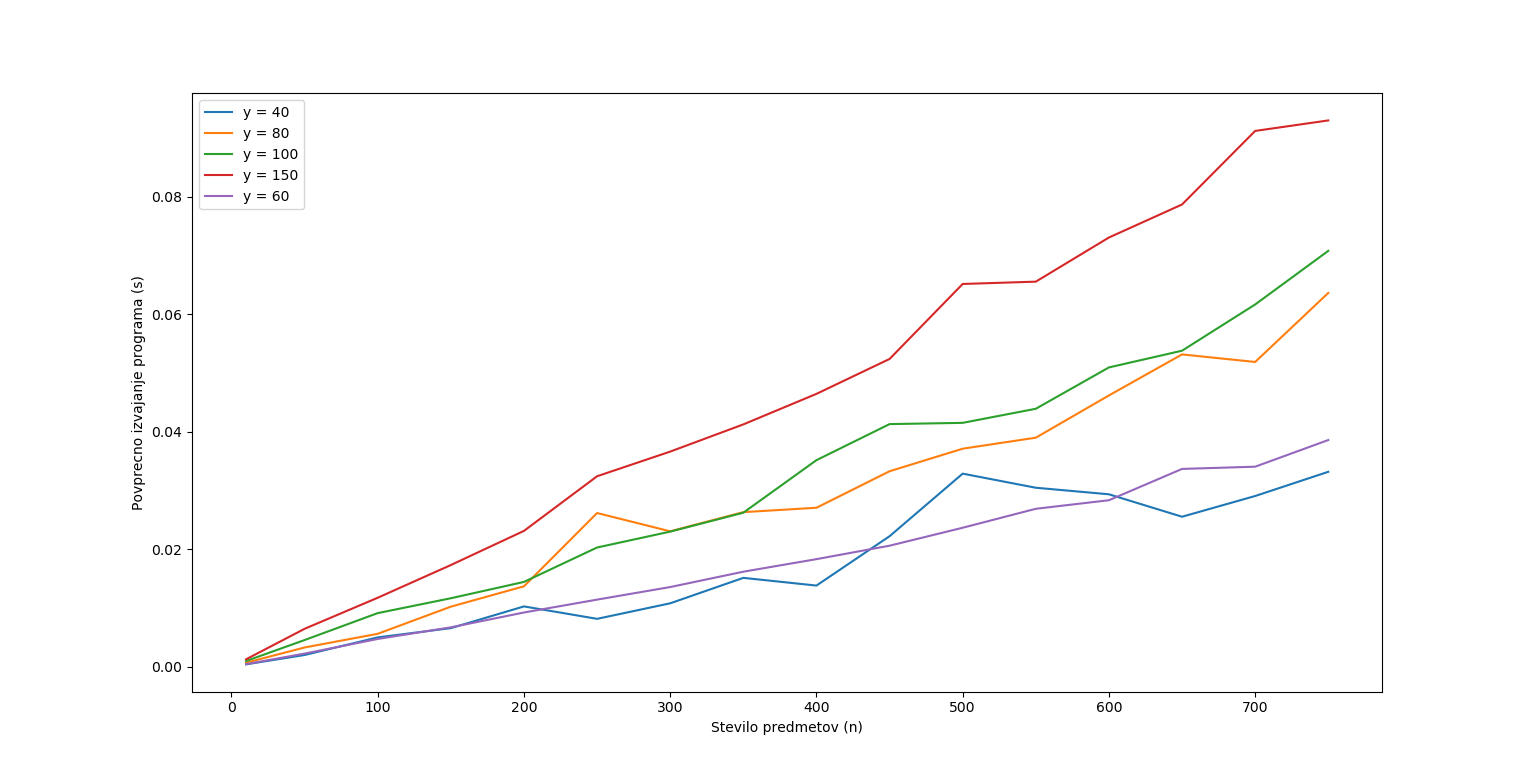
\includegraphics[scale=0.35]{Graf_1_100.png}
    		\caption{Odvisnost od $y$, 100 pon.}
    		\label{fig:graf1_100}
	\end{figure}
	
	\begin{figure}[h]
    	\centering
    		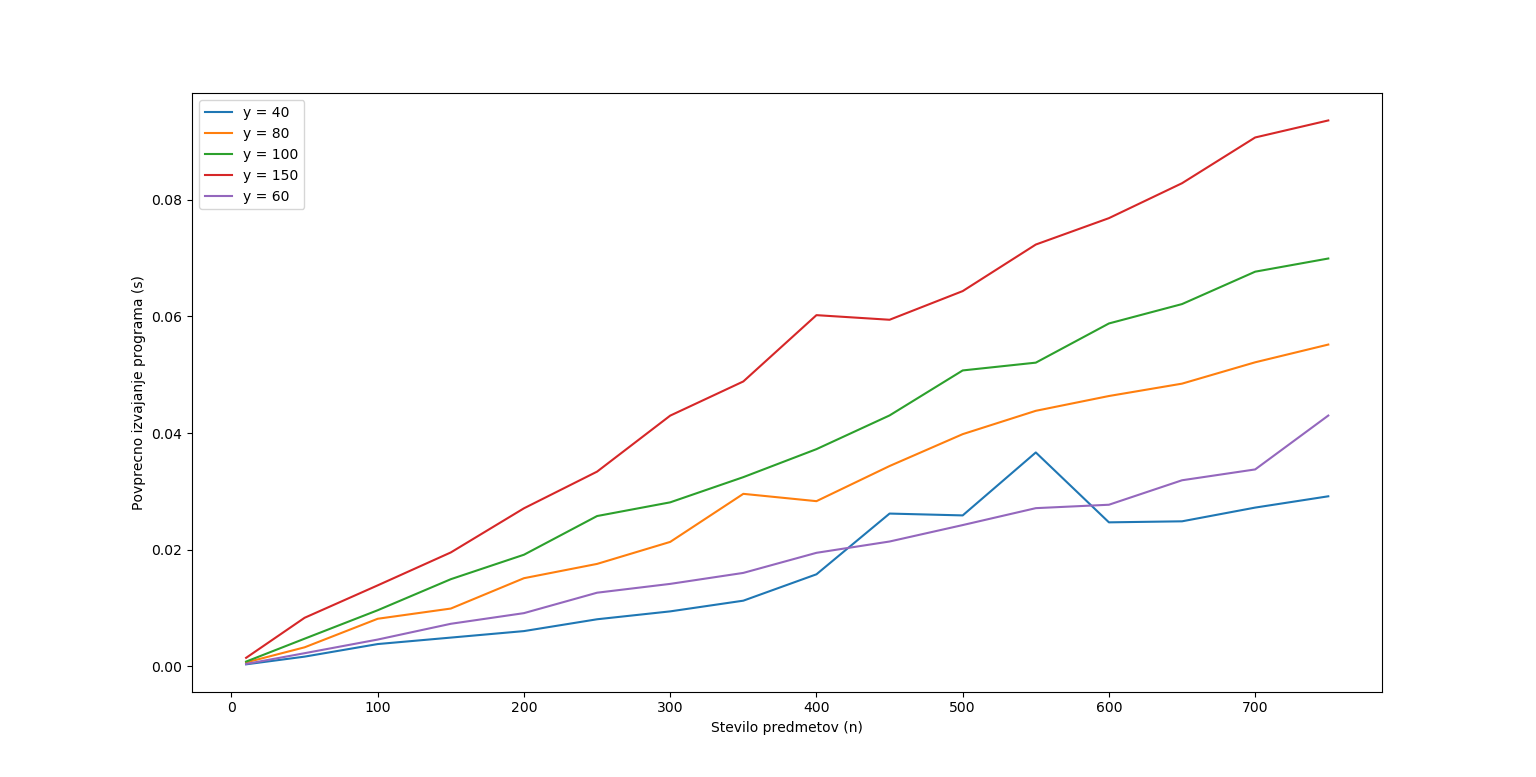
\includegraphics[scale=0.35]{Graf_1_1000.png}
    		\caption{Odvisnost od $y$, 1000 pon.}
    		\label{fig:graf1_1000}
	\end{figure}
	
	\begin{figure}[h]
    	\centering
    		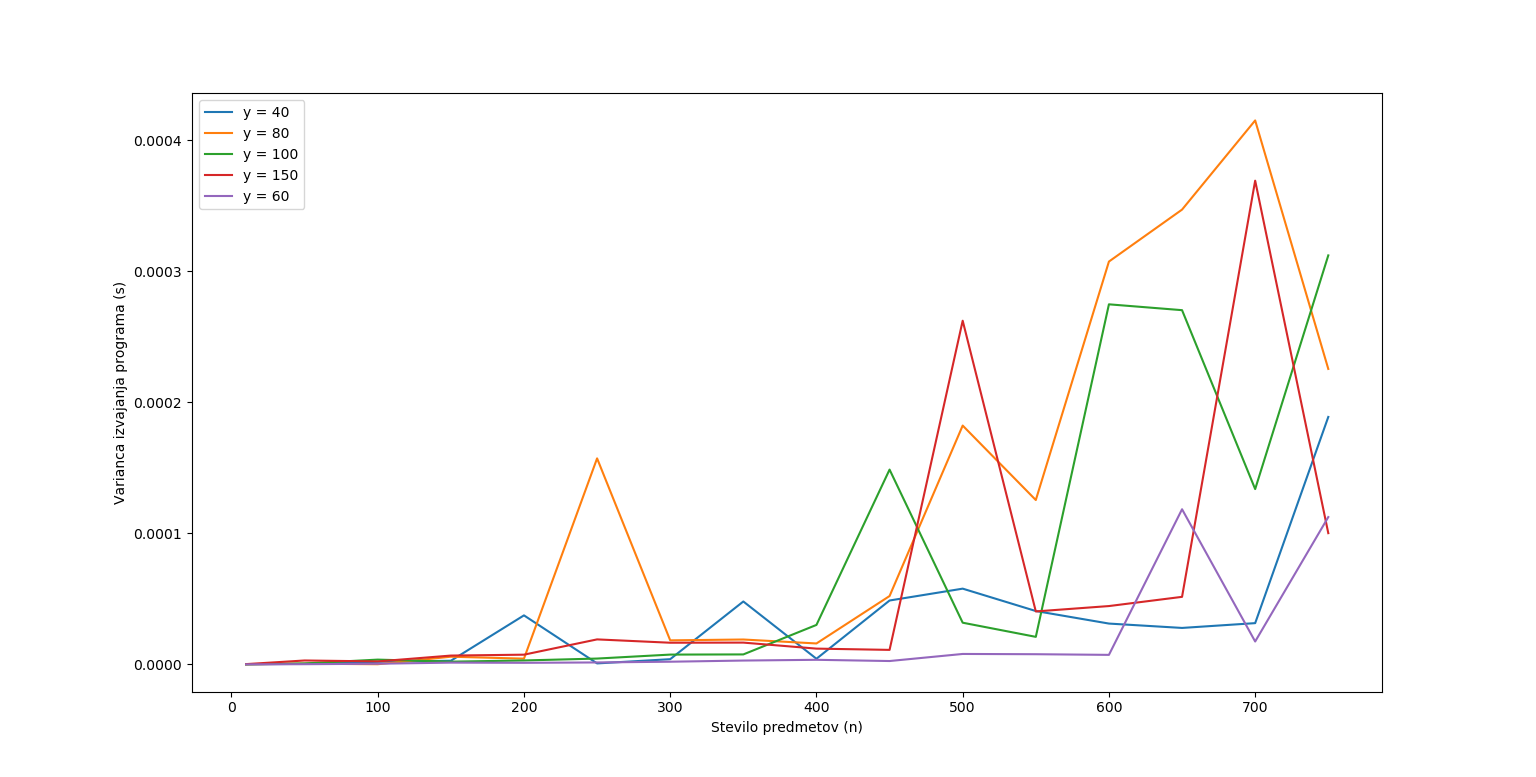
\includegraphics[scale=0.35]{Graf_2_100.png}
    		\caption{Varianca podatkov, 100 pon.}
    		\label{fig:graf3_100}
	\end{figure}
	
	\begin{figure}[h]
    	\centering
    		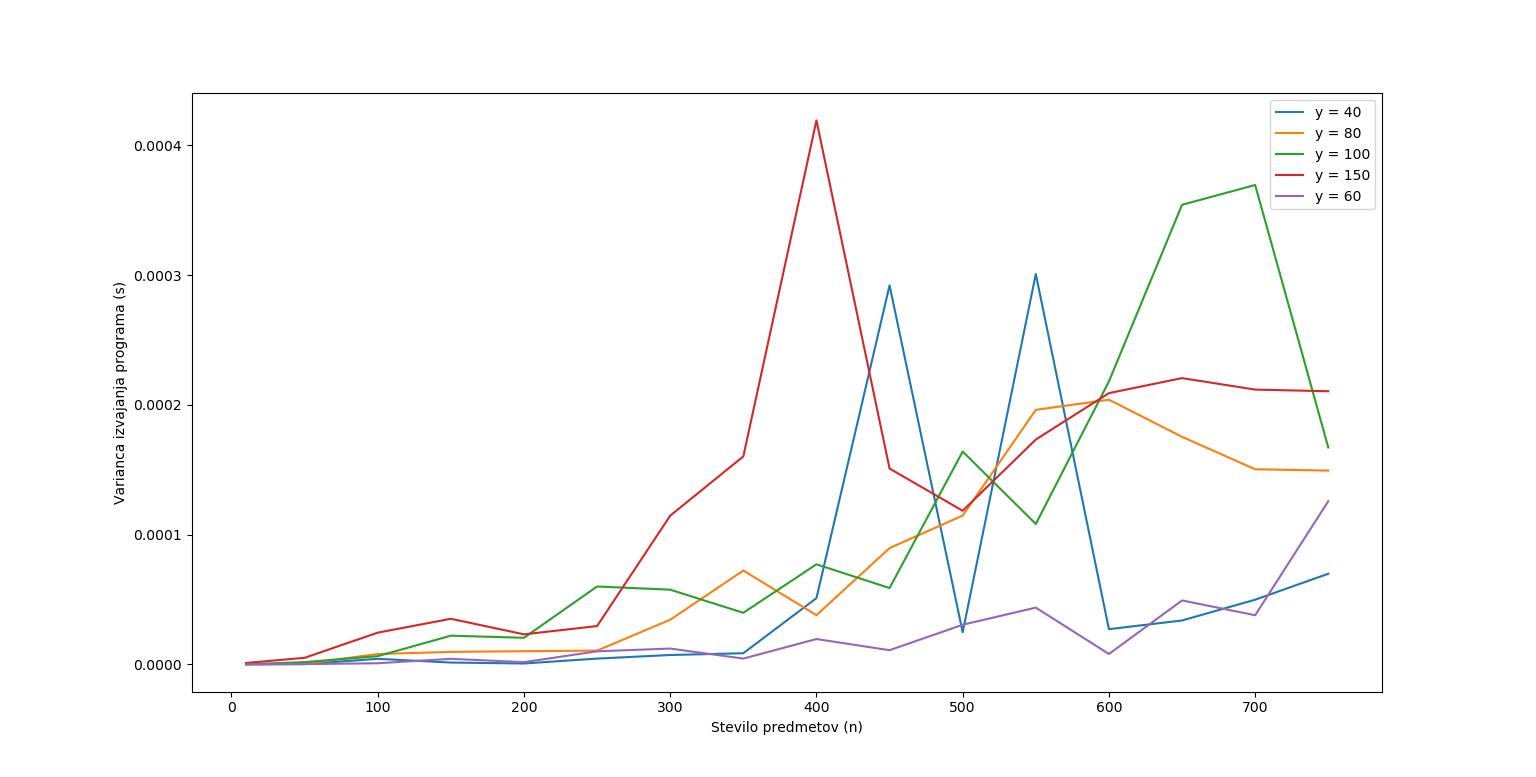
\includegraphics[scale=0.35]{Graf_2_1000.png}
    		\caption{Varianca podatkov, 1000 pon.}
    		\label{fig:graf4_1000}
	\end{figure}
	
	
	\begin{figure}[h]
    	\centering
    		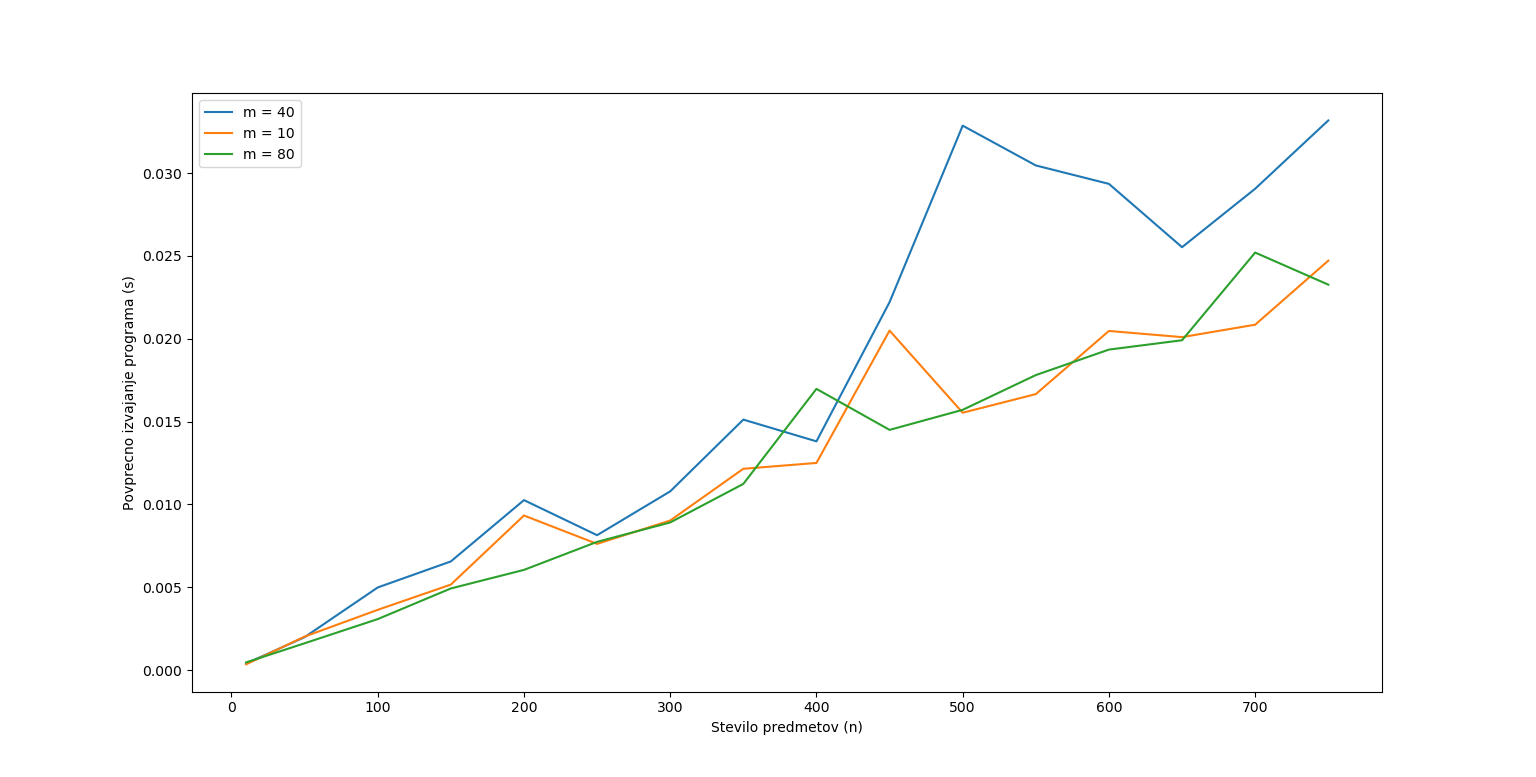
\includegraphics[scale=0.35]{Graf_3_100.png}
    		\caption{Odvisnost od $m$, 100 pon.}
    		\label{fig:graf5_100}
	\end{figure}
	
	\begin{figure}[h]
    	\centering
    		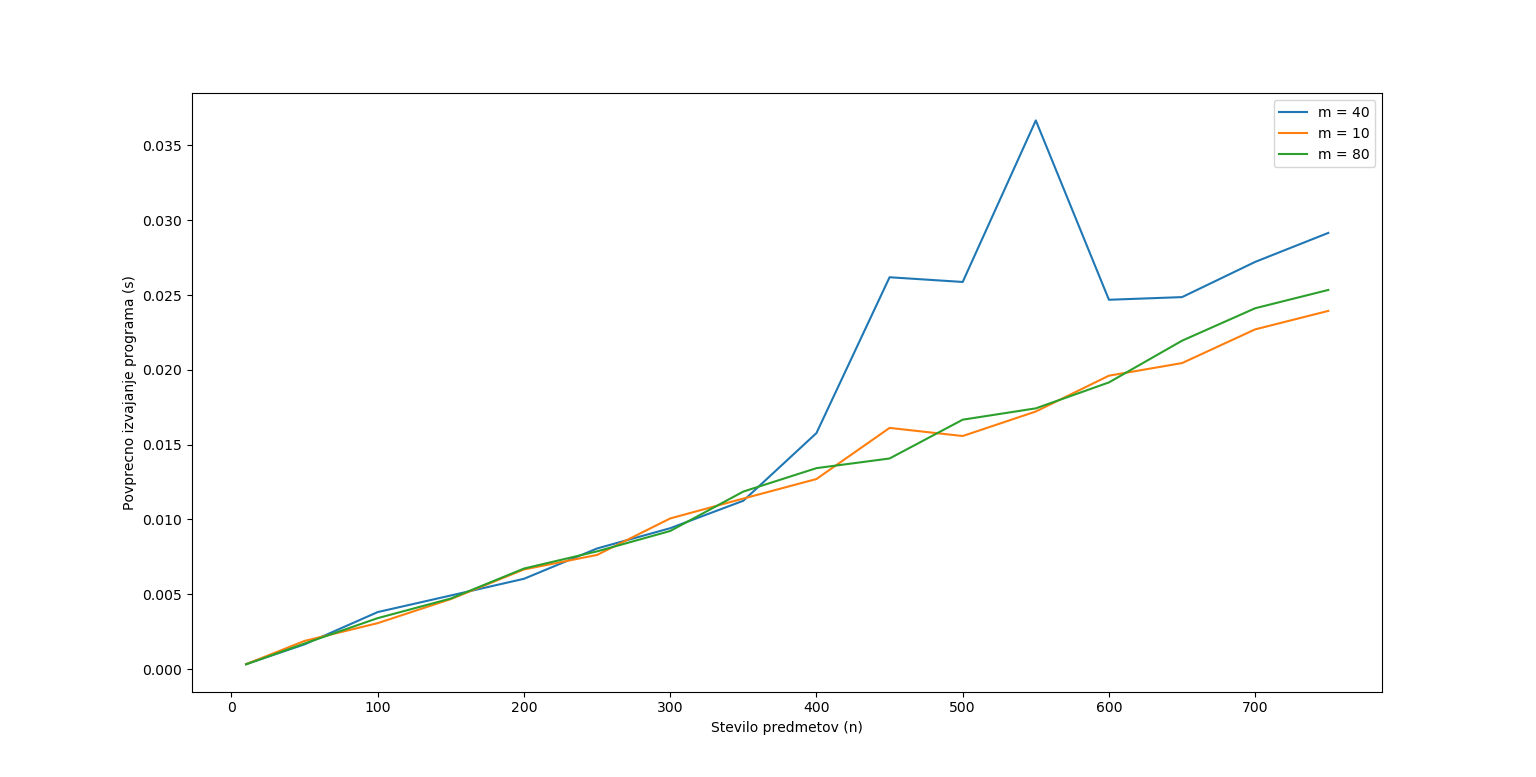
\includegraphics[scale=0.35]{Graf_3_1000.png}
    		\caption{Odvisnost od $m$, 1000 pon.}
    		\label{fig:graf6_1000}
	\end{figure}
	
		\clearpage
		
% VIRI	
		\begin{thebibliography}{9}
		\addcontentsline{toc}{section}{Literatura}
		
			\bibitem{Brotcorne,Hanafi,Mansi2009} L. Brotcorne, S. Hanafi, R. Mansi (2009).
			\textit{A dynamic programming algorithm for the bilevel knapsack problem} Elsevier: Operations Research Letters 37, 215–218.
			
    			\bibitem{Dempe,Richter2000} S. Dempe, K. Richter (2000). 
			\textit{Bilevel programming with Knapsack constraint} European Newspaper of Operations Research 8, 93–107.
			
		\end{thebibliography}
	
	
	
	
\end{document}
